\paragraph{\trPointedDisc。}\label{sub:pointed-discs}
我们现在把讨论限制在与\trFukayaCategory{}有关的那一类\trSurface{}上。一个\textbf{$(d+1)$ \trPointedDisc}%
（(d+1)-pointed disc），$d\ge 0$，是一个\trPointedBoundary\trRiemann\trSurface{}$S$，其\trCompactification{}$\hat{S}\cong D$
是一个\trDisk，并且它恰有一个无穷远处的\trIncomingPoint{}与 $d$ 个\trOutgoingPoint。我们的约定是：给诸
无穷远点编号时，遵循它们沿\trDisk{}边界的\trCyclicOrder，使得\trIncomingPoint{}为 $\Sigma^-=\{\zeta_0\}$，而诸%
\trOutgoingPoint{}为 $\Sigma^+=\{\zeta_1,\ldots,\zeta_d\}$；若 $S$ 带\trStriplikeEnd，我们就相应地把这些端编号为
$\epsilon_0,\ldots,\epsilon_d$。$\partial S$ 的诸\trConnectedComponent{}将记作 $C_0,\ldots,C_d$，同样遵循\trCyclicOrder，且
$\zeta_0$ 位于 $C_d$ 与 $C_0$ 之间（$d=2$ 的情形见\cref{fig:pointed-disc}）。若 $S$ 带\trLagrange\trLabel，则它们相应
地记作 $L_0,\ldots,L_d$。与诸无穷远点相配的\trLagrange\trSubmanifold{}对即为
\begin{equation}\label{eq:lagrangian-pairs}
(L_{\zeta_k,0},L_{\zeta_k,1})=
\begin{cases}
(L_0,L_d) & k=0,\\
(L_{k-1},L_k) & k>0.
\end{cases}
\end{equation}
\begin{figure}[htbp]
\centering
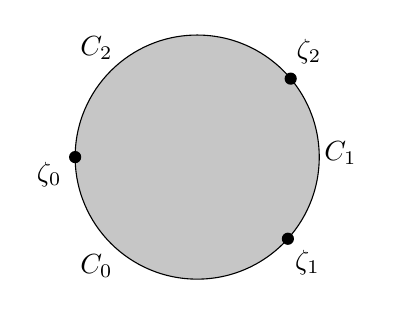
\begin{tikzpicture}[line cap=round,line join=round]
\draw[fill=gray!45] (0,0) circle (1.55);
\fill (180:1.55) circle (2.2pt);
\fill (-42:1.55) circle (2.2pt);
\fill (40:1.55) circle (2.2pt);
\node at (-1.88,-0.22) {$\zeta_0$};
\node at (1.40,-1.34) {$\zeta_1$};
\node at (1.42,1.34) {$\zeta_2$};
\node at (-1.28,1.38) {$C_2$};
\node at (1.82,0.05) {$C_1$};
\node at (-1.28,-1.38) {$C_0$};
\end{tikzpicture}
\caption{}\label{fig:pointed-disc}
\end{figure}
在\emph{稳定范围} $d\ge 2$ 内，$(d+1)$ \trPointedDisc{}没有非平凡的\trAutomorphism，而且存在它们的一个%
\trUniversal\trFamily，记为
\begin{equation}\label{eq:universal-family}
\scr{S}^{d+1}\longrightarrow\scr{R}^{d+1}.
\end{equation}
其构造直截了当：令 $\mathrm{Conf}_{d+1}(\partial D)\subset(\partial D)^{d+1}$ 为由\trCircle{}上的 $(d+1)$ 元点组组成的%
\trConfigurationSpace，其编号与它们的\trCyclicOrder\trCompatible。$\mathrm{Aut}(D)\cong\mathrm{PSL}_2(\RR)$ 自由且\trProper{}地
作用于这个\trConfigurationSpace，于是令
\begin{equation}\label{eq:universal-disc-base}
\scr{R}^{d+1}=\mathrm{Conf}_{d+1}(\partial D)\,/\,\mathrm{Aut}(D),
\qquad
\hat{\scr{S}}^{d+1}=\mathrm{Conf}_{d+1}(\partial D)\times_{\mathrm{Aut}(D)}D.
\end{equation}
\trProjection{}$\hat{\scr{S}}^{d+1}\to\scr{R}^{d+1}$ 容许\trSection{}$\zeta_k([z_0,\ldots,z_d])=[z_0,\ldots,z_d,z_k]$；按照一般的做法，
我们令 $\scr{S}^{d+1}=\hat{\scr{S}}^{d+1}\setminus\bigcup_k\zeta_k(\scr{R}^{d+1})$。\trRiemann\trUniformization（以带参数的
形式）表明\eqref{eq:universal-family} 确实是一个\trUniversal\trFamily，其含义是：每一个 $(d+1)$%
\trPointedDisc{}的\trFamily{}都是 $\scr{S}^{d+1}$ 经由唯一一个从其基到 $\scr{R}^{d+1}$ 的\trSmooth{}映射的%
\trPullback。与之类似的无穷小结果同样不难证明，它说\eqref{eq:universal-family} 是无穷小\trMiniversal{}的。
把带\trStriplikeEnd{}的一个\textbf{\trUniversal{}选取}（universal choice of strip-like ends）定义为：对每个
$d\ge 2$，为 $\scr{S}^{d+1}\to\scr{R}^{d+1}$ 选定一组\trStriplikeEnd{}$\{\epsilon^{d+1}_{k}\}_{0\le k\le d}$。当然，它是%
\trUniversal{}的，其含义是：任何 $(d+1)$ \trPointedDisc{}的\trFamily{}都经由其\trClassifyingMap{}继承%
\trStriplikeEnd。
